\begin{frame}
  \frametitle{Maximizing preserved variance}
  %% \framesubtitle{}

  \begin{itemize}
  \item In our example, we want to find the axis $\vv_1$ that preserves the
    largest amount of variance by maximizing $\vv_1^T \mathbf{C} \vv_1$
  \item<2-> For higher-dimensional data set, we also want to find the\\ axis
    $\vv_2$ with the second largest amount of variance, etc.
    \begin{itemize} 
    \item[\hand] Should not include variance that has already been accounted for:
      $\vv_2$ must be orthogonal to $\vv_1$, i.e.\ $\sprod{\vv_1}{\vv_2} = 0$
    \end{itemize}
  \item<3-> Orthogonal dimensions $\vv[1], \vv[2], \ldots$ \h{partition} variance:
    \[
    \sigma^2 = \sigma_{\vv[1]}^2 + \sigma_{\vv[2]}^2 + \ldots
    \]
  \item<4-> Useful result from linear algebra: every symmetric matrix
    $\mathbf{C} = \mathbf{C}^T$ has an \h{eigenvalue decomposition} with
    orthogonal \hh{eigenvectors} $\va_1, \va_2, \dots, \va_n$ and
    corresponding \hh{eigenvalues} $\lambda_1\geq \lambda_2\geq \dots \geq
    \lambda_n$
  \end{itemize}
\end{frame}

\begin{frame}
  \frametitle{Eigenvalue decomposition}
  %% \framesubtitle{}

  \begin{itemize}
  \item The eigenvalue decomposition of $\mathbf{C}$ can be written in the
    form
    \[
    \mathbf{C} = \mathbf{U}\cdot \mathbf{D}\cdot \mathbf{U}^T
    \]
    where $\mathbf{U}$ is an orthogonal matrix of eigenvectors (columns)
    and $\mathbf{D} = \mathop{\text{Diag}}(\lambda_1, \dots, \lambda_n)$ a diagonal
    matrix of eigenvalues
    \begin{small}
      \[
      \mathbf{U} =
      \begin{bmatrix}
        \vdots & \vdots & & \vdots \\
        \vdots & \vdots & & \vdots \\
        \va_1 & \va_2 & \cdots & \va_n \\
        \vdots & \vdots & & \vdots \\
        \vdots & \vdots & & \vdots
      \end{bmatrix}
      \qquad \mathbf{D} =
      \begin{bmatrix}
        \lambda_1 & & & \\
        & \lambda_2 & & & \\
        & & \ddots & & \\
        & & & \ddots & \\
        & & & & \lambda_n
      \end{bmatrix}
      \]
    \end{small}
    \begin{itemize}
    \item note that both $\mathbf{U}$ and $\mathbf{D}$ are $n\times n$ square matrices
    \end{itemize}
  \end{itemize}
\end{frame}

\begin{frame}
  \frametitle{The PCA algorithm}
  %% \framesubtitle{}

  \begin{itemize}
  \item With the eigenvalue decomposition of $\mathbf{C}$, we have 
    \[
    \sigma_{\vv}^2 = \vv^T \mathbf{C} \vv 
    = \vv^T \mathbf{U} \mathbf{D} \mathbf{U}^T \vv 
    = (\mathbf{U}^T \vv)^T \mathbf{D} (\mathbf{U}^T \vv) 
    = \vy^T \mathbf{D} \vy
    \]
    where $\vy = \mathbf{U}^T \vv$ = $[y_1, y_2, \ldots, y_n]^T$ are the
    coordinates of $\vv$ in the Cartesian basis formed by the eigenvectors of
    $\mathbf{C}$
  \item<2-> $\norm{\vy} = 1$ since $\mathbf{U}^T$ is an isometry (orthogonal matrix)
  \item<2-> We therefore want to maximize 
    \[
    \vv^T \mathbf{C} \vv = \lambda_1 (y_1)^2 + \lambda_2 (y_2)^2 \dots + \lambda_n (y_n)^2
    \]
    under the constraint $(y_1)^2 + (y_2)^2 + \dots + (y_n)^2 = 1$
  \item<3-> Solution: $\vy = [1, 0, \dots, 0]^T$ (since $\lambda_1$ is the
    largest eigenvalue)
  \item<3-> This corresponds to $\vv = \va_1$ (the first eigenvector of
    $\mathbf{C}$) and a preserved amount of variance given by $\sigma_{\vv}^2
    = \va_1^T \mathbf{C} \va_1 = \lambda_1$
  \end{itemize}
\end{frame}

\begin{frame}
  \frametitle{The PCA algorithm}
  %% \framesubtitle{}

  \begin{itemize}
  \item In order to find the dimension of second highest variance,\\
    we have to look for an axis $\vv$ orthogonal to $\va_1$
    \begin{itemize}
    \item[\hand] $\mathbf{U}^T$ is orthogonal, so the coordinates $\vy =
      \mathbf{U}^T \vv$ must be orthogonal to first axis $[1, 0, \dots, 0]^T$,
      i.e.\ $\vy = [0, y_2, \dots, y_n]^T$
    \end{itemize}
  \item<2-> In other words, we have to maximize
    \[
    \vv^T \mathbf{C} \vv = \lambda_2 (y_2)^2 \dots + \lambda_n (y_n)^2
    \]
    under constraints $y_1 = 0$ and $(y_2)^2 + \dots + (y_n)^2 = 1$
  \item<3-> Again, solution is $\vy = [0, 1, 0, \dots, 0]^T$, corresponding to the
    second eigenvector $\vv = \va_2$ and preserved variance $\sigma_{\vv}^2 =
    \lambda_2$
  \item<4-> Similarly for the third, fourth, \ldots\ axis
  \end{itemize}
\end{frame}

\begin{frame}
  \frametitle{The PCA algorithm}
  %% \framesubtitle{}

  \begin{itemize}
  \item The eigenvectors $\va_i$ of the covariance matrix $\mathbf{C}$ are
    called the \h{principal components} of the data set
  \item The amount of variance preserved (or ``explained'') by the $i$-th
    principal component is given by the eigenvalue $\lambda_i$
  \item Since $\lambda_1 \geq \lambda_2 \geq \dots \geq \lambda_n$, the first
    principal component accounts for the largest amount of variance etc.
  \item Coordinates of a point $\vx$ in PCA space are given by $\mathbf{U}^T
    \vx$ (note: these are the projections on the principal components)
  \item For the purpose of ``noise reduction'', only the first $n' < n$
    principal components (with highest variance) are retained, and the other
    dimensions in PCA space are dropped
    \begin{itemize}
    \item[\hand] i.e.\ data points are projected into the subspace $V$ spanned
      by the first $n'$ column vectors of $\mathbf{U}$
    \end{itemize}
  \end{itemize}
\end{frame}

\begin{frame}[c]
  \frametitle{PCA example}
  %% \framesubtitle{}

  \ungap
  \begin{center}
    \only<beamer:1| handout:0>{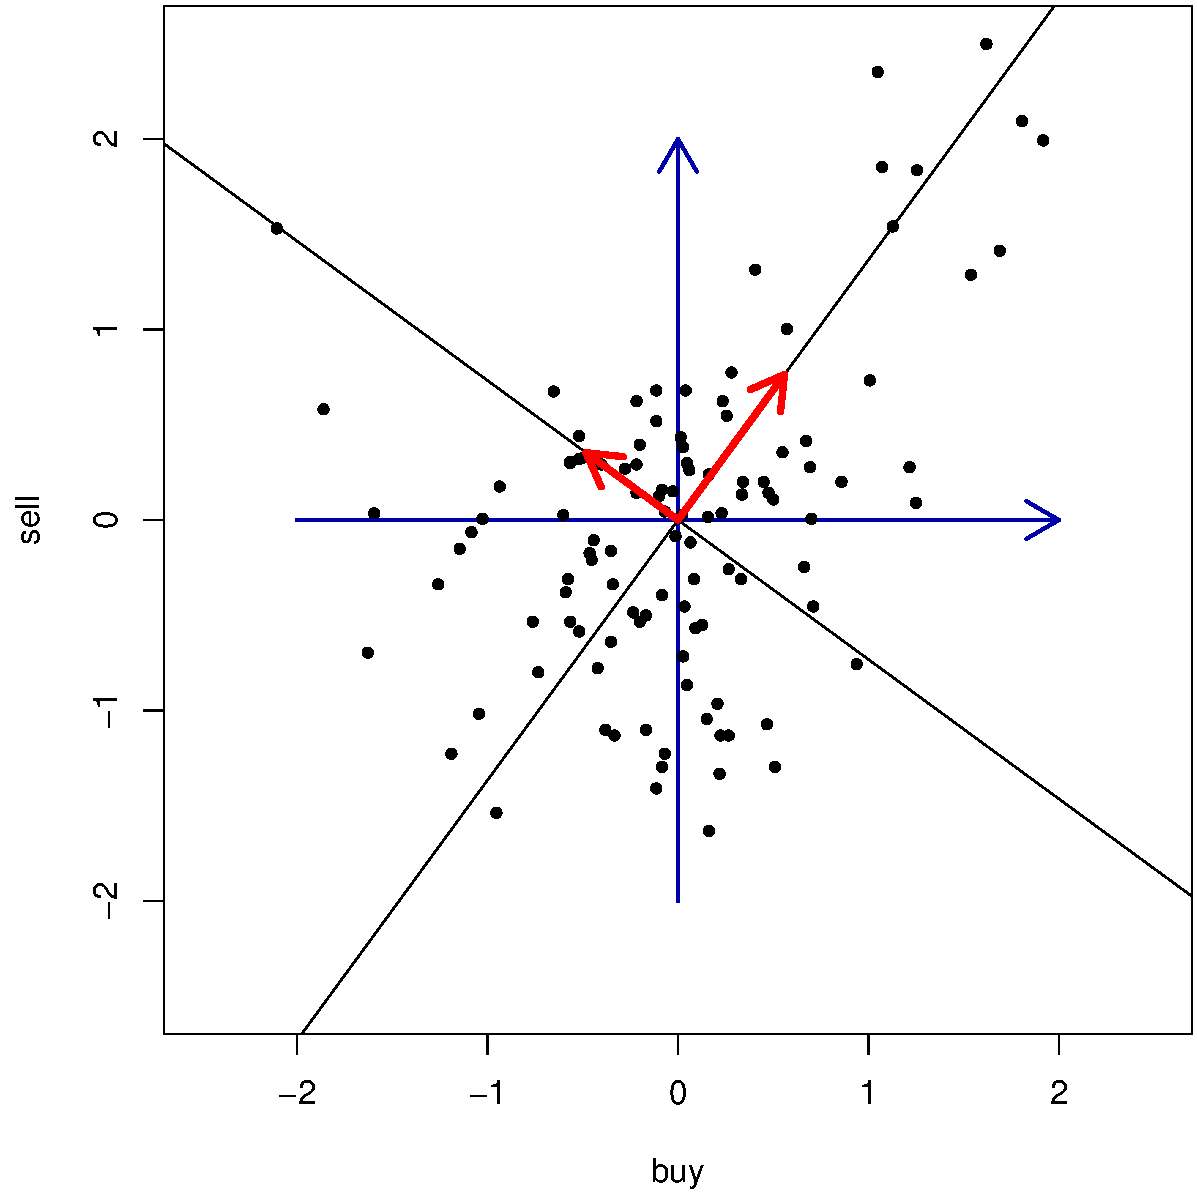
\includegraphics[width=8cm]{img/3_buy_sell_pca}}%
    \only<beamer:2| handout:1>{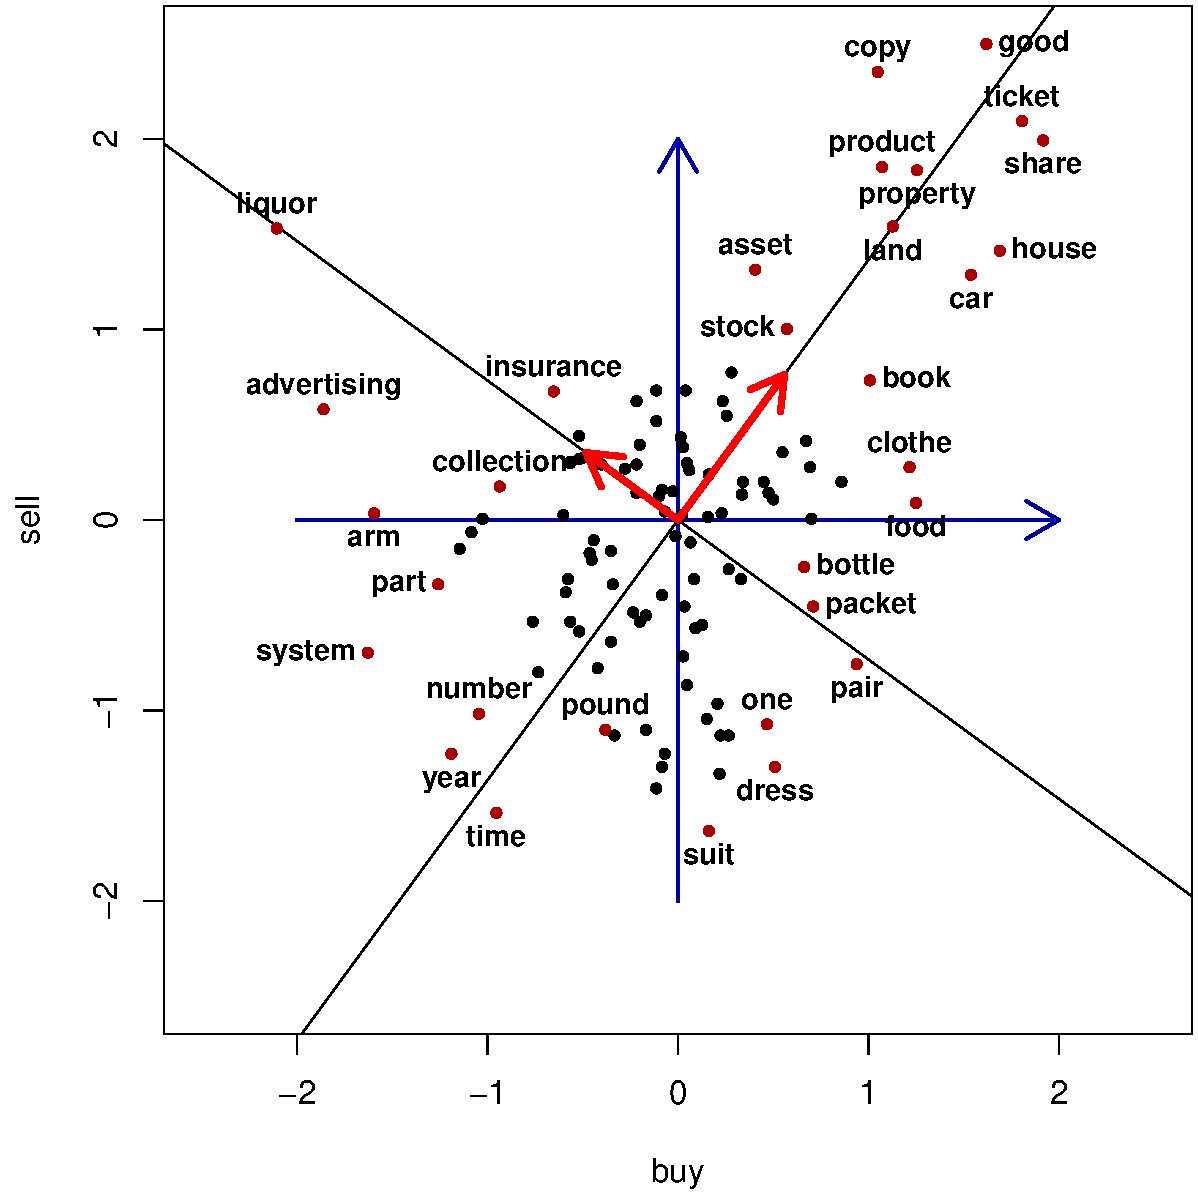
\includegraphics[width=8cm]{img/3_buy_sell_pca_labels}}%
  \end{center}
\end{frame}

%%% Local Variables: 
%%% mode: latex
%%% TeX-master: "../../workspace"
%%% End: 
